\section{Wprowadzenie techniczne}

Zaimplementowany algorytm rozpoznawania kolorów samochodów osobowych opiera swoje działanie na uczeniu maszynowym. We wprowadzeniu przybliżony zostanie koncept uczenia maszynowego, jak i terminologia oraz techniki dotyczące tego zagadnienia. Zagłębiając się dalej w koncepcje stosowane w obszarze uczenia maszynowego, omówiona zostanie zasada działania uczenia opartego o model oraz architektura modelu sieci neuronowej.\\
W dalszym etapie poruszone zostaną techniki optymalizacji wydajności uczenia maszynowego pod kątem wstępnego przetwarzania danych. Przytoczone zostaną metody wstępnego przetwarzania obrazów takie jak segmentacja semantyczna, segmentacja instancyjna i wyodrębnianie cech znaczących.\\
Na koniec rozdziału zostanie omówiona kwestia statystyk dotyczących koloru samochodów na polskich drogach oraz używanego w projekcie zbioru danych. Jest on obarczony wieloma problemami, które zostaną przytoczone i omówione.

\subsection{Uczenie maszynowe}
\subsubsection{Definicja}
Uczenie maszynowe można opisać na wiele sposobów, gdyż jest to pojęcie pokrywające szeroki zakres zastosowań i może przyjmować wiele form. Podane zatem zostaną dwa niezależne sformułowania definicji uczenia maszynowego. Pierwsza, opisowa, w przystępny sposób przybliża koncepcję uczenia maszynowego. Druga zaś, to czysto inżynierska forma definicji.

\begin{description}
\item "\textbf{Uczenie maszynowe} to używanie matematycznych modeli danych w celu ułatwienia komputerowi uczenia się bez bezpośrednich instrukcji. Jest ono traktowane jako podzbiór sztucznej inteligencji. Algorytmy używane w uczeniu maszynowym umożliwiają określanie wzorców w danych. Wzorce te są następnie używane do tworzenia modelu danych, który pozwala przewidywać. Dokładność wyników uczenia maszynowego zwiększa się wraz z upływem czasu i wzrostem ilości danych - podobnie jak u ludzi.

Elastyczność uczenia maszynowego sprawia, że staje się ono świetnym wyborem w scenariuszach, w których dane lub charakter żądania bądź zadania stale się zmieniają, albo w sytuacjach, w których zakodowanie rozwiązania byłoby w praktyce niemożliwe." \cite{microsoftazure}.

\item Program komputerowy \textbf{uczy się} z doświadczenia \textbf{D} na temat zadania \textbf{Z}, jeśli wybrana metryka wydajności \textbf{W} wobec zadania \textbf{Z} jest zwiększana wraz z pozyskiwaniem doświadczenia \textbf{D} \cite{tommitchel}.
\end{description}

Z obu definicji, możemy wywnioskować, że w kontraście do klasycznego podejścia do programowania, uczenie maszynowe wyklucza jawne definiowanie reguł i operacji w celu osiągnięcia danej funkcjonalności algorytmu. Do wyuczenia się sposobu wykonywania zadania system iteracyjnie wyciąga wnioski z zapewnionych przez programistę danych.\\
Porównanie klasycznego programowania i uczenia maszynowego obrazują dwa poniższe rysunki.

\begin{figure}[h!]
    
    \begin{center}
        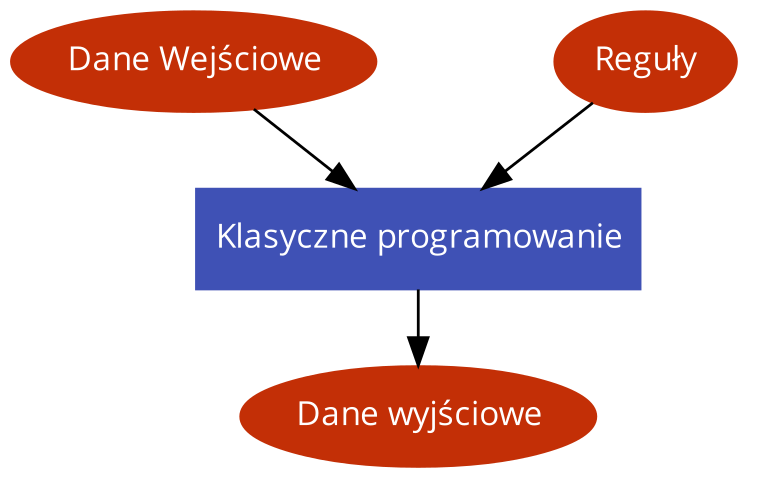
\includegraphics[scale=0.55]{img/Classic.png}
        \caption{Klasyczne programowanie}
        \label{fig:Klasyczne programowanie}    
    \end{center}
    
    \begin{center}
        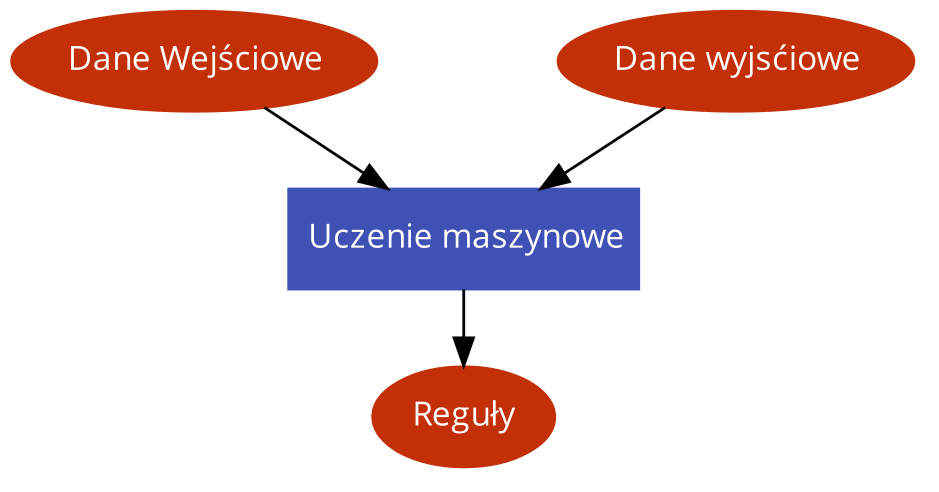
\includegraphics[scale=0.52]{img/ML.png}
        \caption{Uczenie maszynowe}
        \label{fig:Uczenie maszynowe}
    \end{center}
    
\end{figure}

\subsubsection{Klasyfikacja}

Rozróżnienie poszczególnych rodzajów uczenia maszynowego pod względem sposobów działania jest ważne, ponieważ ich zastosowania mogą się znacząco różnić. Systematykę metod uczenia maszynowego można prowadzić pod wieloma względami. Najczęściej wyróżniane są trzy aspekty dzielące techniki uczenia.

Po pierwsze, rozróżniamy metody uczenia ze względu na to czy występuje w nich potrzeba nadzoru ludzkiego. \textbf{Nadzór} w tym wypadku sprowadza się do tego, czy dane uczące posiadają etykiety. \textbf{Etykiety}, czyli oczekiwany wynik (wyjście) odpowiadający konkretnej, uczącej danej wejściowej. Wyróżniamy systemy:

\begin{description}
\item \textbf{Nadzorowane} - dane uczące sporządzone na potrzeby stworzenia algorytmu, oprócz danych wejściowych zawierają rozwiązania. Inaczej mówiąc, zawierają oczekiwane dane wyjściowe.\\Powszechnym zadaniem algorytmów nadzorowanych jest klasyfikacja obiektów oraz regresja. \textbf{Klasyfikacja} polega na przypisaniu obiektu do danej klasy. \textbf{Regresja} to inaczej przewidywanie liczbowego celu.\\ Popularne algorytmy wykorzystujące nadzorowane uczenie maszynowe to:
    \begin{itemize}
        \item Najbliższych sąsiadów (K-nn)
        \item Regresja liniowa
        \item Maszyna wektorów nośnych (SVM)
        \item Drzewa decyzyjne
        \item Las losowy
        \item Sieci neuronowe
    \end{itemize}
    
    \begin{figure}[h!]
    \begin{center}
        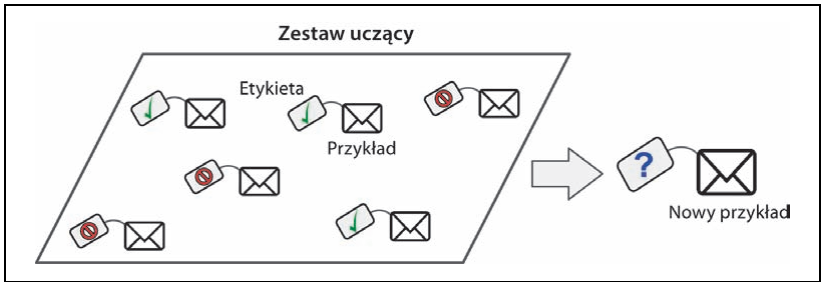
\includegraphics[scale=0.75]{img/oreily.png}
        \caption{Uczenie nadzorowane \cite{oreilly}}
        \label{fig:nadzorowane}    
    \end{center}
    
\end{figure}
\item \textbf{Nienadzorowane} - dane uczące nie posiadają etykiet. Działające na tej podstawie algorytmy są często stosowane do wizualizacji rozkładu danych. Oprócz tego ich typowym zastosowaniem jest wykrywanie anomalii w zbiorach danych. Najpopularniejsze algorytmy związane z nienadzorowanym uczeniem maszynowym to:
    \begin{itemize}
        \item Algorytm centroid-ów (K-Means)
        \item segmentacja danych punktowych oraz rastrowych (DBSCAN)
        \item Grupowanie hierarchiczne (HCA)
    \end{itemize}
    
    \begin{figure}[h!]
    
    \begin{center}
        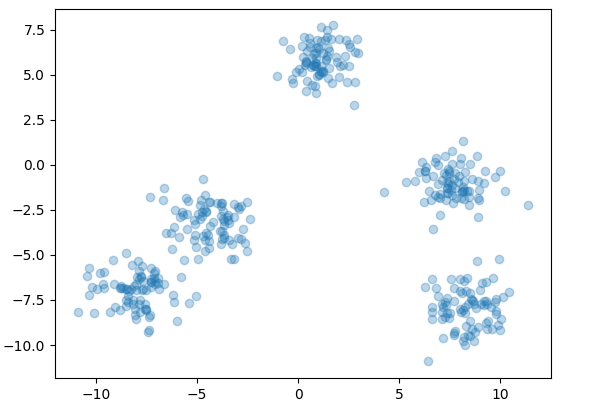
\includegraphics[scale=0.76]{img/unsupervised.png}
        \caption{Zbiór danych bez etykiet}
        \label{fig:nienadzorowane}    
    \end{center}
    
    \begin{center}
        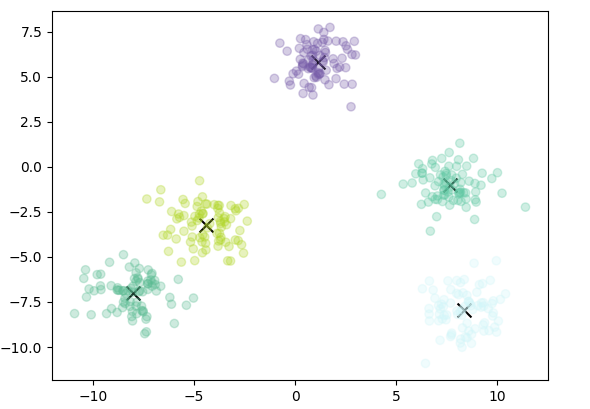
\includegraphics[scale=0.76]{img/kmeans.png}
        \caption{Wizualizacja wyniku algorytmu centroid-ów}
        \label{fig:kmeans}
    \end{center}
    
\end{figure}

\pagebreak
    
\item \textbf{Pół-nadzorowane} - tylko część danych posiada etykiety. Działanie takiego algorytmu można zobrazować na podstawie działania serwisu zdjęć Google. Wyszukują i grupują one z wszystkich zapisanych zdjęć twarze i grupują je osobami, nie wiedząc kto to jest. Następnie użytkownik sam nadaje etykiety do grup zdjęć na przykład w postaci imion, implementując w ten sposób aspekt pół-nadzoru \cite{oreilly}.  

\item \textbf{Uczenie ze wzmocnieniem} - algorytm sam na podstawie dostępnych danych podejmuje wobec nich działania. Jest on regulowany poprzez system nagród i kar. Gdy akcja, którą wykonał była pożądana - jest on nagradzany. W przeciwnym wypadku jest karany. Ten rodzaj uczenia jest powszechnie stosowany w systemach uczących wykorzystywanych w robotyce. W ten sposób robot stopniowo uczy się wykonywać pożądane przez twórców czynności.
\end{description}

Po drugie, możemy rozróżnić rodzaje uczenia maszynowego ze względu na możliwość ciągłego przyswajania nowych danych.
\begin{description}
\item \textbf{Uczenie przyrostowe} - system jest w stanie przyswajać nowe dane uczące w ciągły sposób w trakcie działania. Jest to najlepsze rozwiązanie dla algorytmów potrzebujących adaptować się do nowych danych, które jeszcze nie powstały. Nieprzerwane przystosowywanie się takiego systemu do nowych danych ciągnie za sobą poważny problem. Może on zatracić pożądaną funkcjonalność z czasem, przez wpływ niskiej jakości danych. Jest to zjawisko zwane \textbf{dryfem}. Twórca algorytmu może mu częściowo zapobiec dobierając odpowiedni \textbf{Współczynnik uczenia}. Dzięki niskiemu współczynnikowi uczenia, wpływ dryfu spowodowany potencjalnie zdegenerowanymi, nowymi danymi jest zmniejszony kosztem wolniejszego przystosowywania się do nowych, potencjalnie pożądanych danych.

    \begin{figure}[h!]
    \begin{center}
        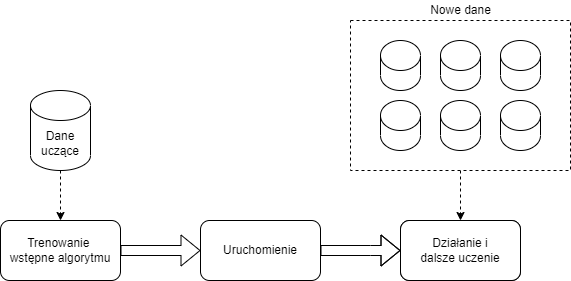
\includegraphics[scale=0.7]{img/przyrostowe.png}
        \caption{Uczenie przyrostowe}
        \label{fig:uczenie_przyrostowe}    
    \end{center}
    \end{figure}

\item \textbf{Uczenie wsadowe} - w procesie uczenia modelu używane są \textbf{wszystkie} dane ze zbioru. 
Każda inicjatywa zmiany działania modelu wymaga jego ponownego, całkowitego wyuczenia. Systemy utylizujące tego typu uczenie, muszą być wyposażone w nietuzinkowe ilości pamięci operacyjnej oraz ogromną moc obliczeniową. Potrzebują one bowiem dużo czasu i zasobów w celu trenowania, zwłaszcza w porównaniu z uczeniem na bieżąco. Algorytmy bazujące na uczeniu przyrostowym mogą ładować kolejne paczki danych uczących, usuwając je, zaraz po użyciu ich w celu uczenia. Ta procedura znacznie zmniejsza zapotrzebowanie sprzętowe.
\end{description}

Na koniec, możemy rozróżnić uczenie maszynowe ze względu na sposób wnioskowania odpowiedzi z danych uczących. Są to:

\begin{description}
\item \textbf{Uczenie z przykładu} - porównujemy nowe instancje danych z wyuczonymi już punktami danych, w ten sposób wnioskując do jakiej grupy danych należy napotkana nowa dana. Aby nie ograniczać algorytmu do odnajdywania odpowiedzi tylko do \underline{identycznych} wejść, jakie posiadał zbiór uczący stosowana jest \textbf{miara podobieństwa}. Pozwala ona na pożądane \textbf{uogólnienie} procesu wnioskowania, biorąc pod uwagę znacznie szerszą gamę danych - te znane oraz grupa danych do nich zbliżonych.

\item \textbf{Uczenie z modelu} - przyjmujemy założenia względem problemu oraz danych wejściowych, wybierając i trenując odpowiednio dobrany \underline{model} (np. regresja liniowa, drzewo decyzyjne, sieć neuronowa i wiele innych). Ucząc model, nadajemy mu zdolność prognozowania na podstawie zależności zachodzących w danych uczących. Powszechnie przyjęte miary pozwalające opisać poprawność działania modelu to \textbf{funkcja dopasowania} oraz \textbf{funkcja kosztu}. Funkcja dopasowania ma za zadanie opisać użyteczność modelu. Uwidocznić to, jak dobrze model współgra z danymi, na podstawie których ma generalizować oraz przewidywać. Funkcja kosztu ma przeciwne zastosowanie. Mierzy ona różnicę pomiędzy oczekiwanymi wynikami, a tymi osiągniętymi przez model.
\end{description}

Wszystkie trzy podziały są od siebie niezależnie i ich mieszanie pomaga osiągnąć różne rezultaty. Dobranie odpowiedniego typu algorytmu jest często kluczowe w celu optymalizacji skuteczności i wydajności jego działania. Dla każdego problemu ze sfery uczenia maszynowego istnieje kilka podejść, które bardziej pasują do natury zagadnienia i będą działać lepiej niż pozostałe. Jeśli potrafimy wysnuć wnioski i skutecznie rozpracować problem, który chcemy rozwiązać uczeniem maszynowym, możemy przyjąć pewne założenia. Pomagają one z doborem strategii działania oraz implementacji systemu bez potrzeby empirycznego szukania najlepszej konfiguracji.

\pagebreak

\subsection{Sieć neuronowa}

\subsubsection{Historia}
\begin{description}
 \item "Początki sztucznej inteligencji sięgają lat czterdziestych ubiegłego stulecia kiedy to opracowano model neuronu w mózgu ludzkim i zwierzęcym (McCulloch i Pitts, 1943) oraz wyjaśniono mechanizm zapamiętywania informacji przez sieć biologiczną. Dalszy rozwój tej nauki zaowocował zaprojektowaniem i zbudowaniem przez Rosenblatta (1958) sztucznej sieci neuronowej zwanej perceptronem. Był to elementarny system wizualny, który mógł być nauczony rozpoznawania ograniczonej klasy wzorów. W tych latach próbowano też pierwszych zastosowań komputerów między innymi do przewidywania pogody, identyfikacji formuł matematycznych, czy analizy elektrokardiogramu.
 
 \item Po publikacji w 1969 książki Minsky'ego i Paperta, w której udowodnili, że jednowarstwowe sieci mają skończone zastosowania, nastąpił odwrót od sieci neuronowych w kierunku systemów ekspertowych. Powrót zainteresowania w połowie lat osiemdziesiątych zapoczątkowały prace ukazujące, że wielowarstwowe, nieliniowe sieci neuronowe nie mają ograniczeń. W tym też okresie rozpoczął się rozwój neurokomputerów, na który także miał wpływ postęp technologii wytwarzania układów scalonych VLSI. Ważnym osiągnięciem są także różnego rodzaju metody uczenia sieci wielowarstwowych np. algorytm wstecznej propagacji błędów." \cite{wstepAGH}.
\end{description}

\subsubsection{Definicja}
\begin{description}
\item "\textbf{Sieci neuronowe}, znane również jako sztuczne sieci neuronowe (ANN) lub symulowane sieci neuronowe (SNN) są częścią funkcji uczenia maszynowego i stanowią podstawę algorytmów uczenia głębokiego. Ich nazwa i struktura są wzorowane na ludzkim mózgu i naśladują sposób, w jaki biologiczne neurony komunikują się między sobą.

Sztuczne sieci neuronowe (ANN) składają się z warstw węzłów, obejmujących warstwę wejściową, jedną lub więcej warstw ukrytych oraz warstwę wyjściową. Każdy węzeł (sztuczny neuron) łączy się z innym i ma powiązaną wagę oraz próg. Jeśli wyjście dowolnego pojedynczego węzła przekracza określoną wartość progową, węzeł ten jest aktywowany podczas wysyłania danych do kolejnej warstwy sieci. W przeciwnym razie żadne dane nie są przekazywane do następnej warstwy sieci." \cite{ibm}.
\end{description}

\pagebreak

\begin{figure}[h!]
    \begin{center}
        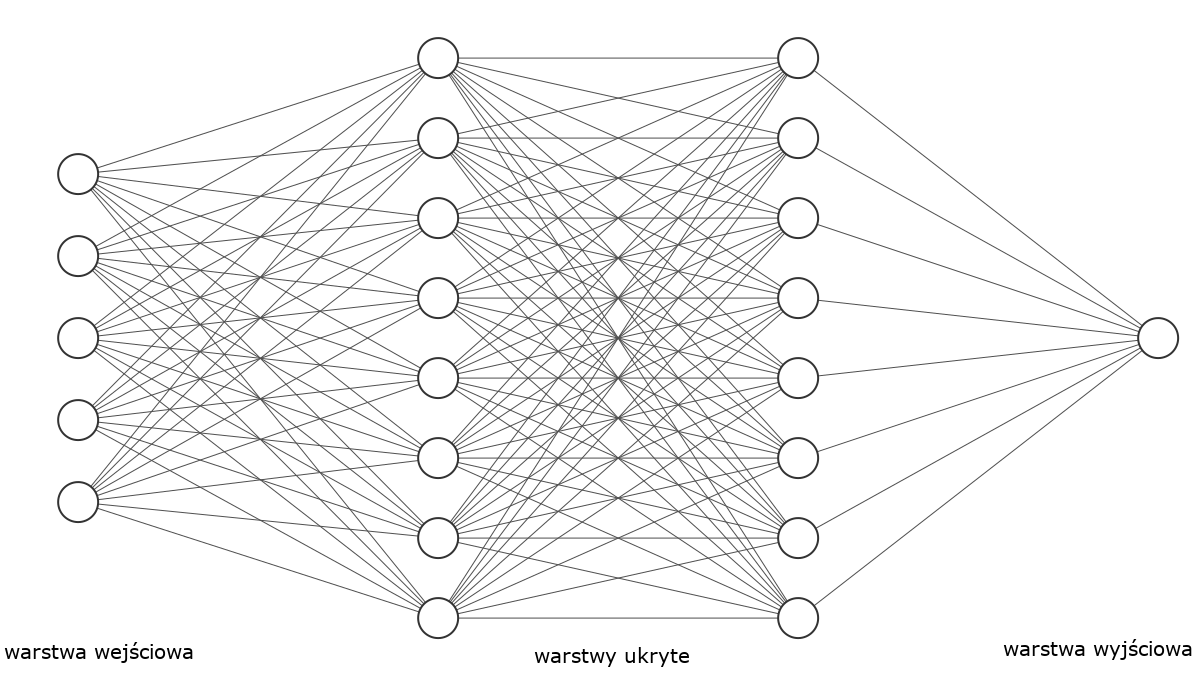
\includegraphics[scale=0.52]{img/nn.png}        
    \end{center}
    \caption{Sieć neuronowa MLP (Perceptron wielowarstwowy)\protect\footnotemark}
    \label{fig:sieć neuronowa}
\end{figure}

\footnotetext{Obraz wygenerowany dzięki narzędziu dostępnemu pod adresem: \url{https://alexlenail.me/NN-SVG}}

\subsubsection{Warstwy sieci neuronowej}
\begin{itemize}
    \label{itm:warstwy}
    \item \textbf{Warstwa wejściowa} - jest nią zawsze pierwsza warstwa. 
    "\null{}Zbiera dane i przekazuje je dalej. [...] Analogicznie jak w przypadku obrazów rejestrowanych np. przez nerwy wzrokowe u człowieka – trafiają do niej nieprzetworzone dane wejściowe" \cite{sztucznainteligencja}
    \item \textbf{Warstwy ukryte} - kluczowe w procesie uczenia. To w nich, szukane są powiązania między poszczególnymi aspektami danej, wprowadzonej z warstwy wejściowej poprzez miary wag, odchyleń i wartości progowych
    \item \textbf{Warstwa wyjściowa} - efekt działania naszego modelu. Ilość węzłów tej warstwy zależy od formatu danych wyjściowych, czyli oczekiwanych przez nas wyników działania sieci (na przykład: lista kolorów wraz z prawdopodobieństwami). Dzięki mierzę prawdopodobieństwa wybierany jest przewidziany wynik wyjściowy modelu - standardowo jest to węzeł z najwyższym rezultatem).
\end{itemize}

\pagebreak

\subsubsection{Perceptron}
Działanie sieci neuronowej najlepiej tłumaczyć zaczynając od opisu jego prostszej formy - \textbf{perceptronu}. To twór złożony z jednego lub wielu \underline{neuronów McCullocha-Pittsa}. Najbardziej trywialny wariant - jedno-neuronowy - potrafi dokonać jedynie klasyfikacji binarnej - określić czy parametry wejściowe należą do danej klasy, czy też nie. Aby otrzymać funkcjonalność klasyfikacji wielu klas należy użyć większej ilości neuronów w warstwie wyjściowej.

\begin{figure}[h!]
    \begin{center}
        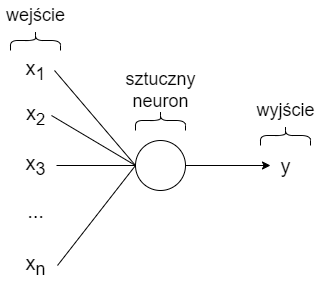
\includegraphics[scale=0.7]{img/perceptron.png}        
    \end{center}
    \caption{Najprostsza forma perceptronu}
    \label{fig:perceptron}
\end{figure}

Bardziej szczegółowy model perceptronu możemy przedstawić zdejmując poziom abstrakcji z neuronu McCullocha-Pittsa. Wtedy model składa się z wejść, ich wag, bloku sumującego, blok aktywacyjnego oraz wyjścia.

\begin{figure}[h!]
    \begin{center}
        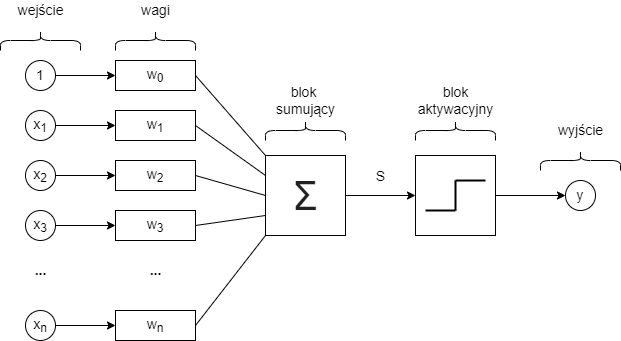
\includegraphics[scale=0.65]{img/perceptron+.png}        
    \end{center}
    \caption{Blokowy schemat perceptronu \cite{wstepAGH}}
    \label{fig:blok_perceptron}
\end{figure}

Działanie tak modelowanego perceptronu charakteryzuję się wzorem:\\

\begin{math}
    \resizebox{0.9\hsize}{!}{$%
    S = \sum_{i = 1}^{m} w_{i}x_{i} + b = w_{1}x_{1} + w_{2}x_{2} + ... + w_{m}x_{m} + b
    $%
    }%
\end{math}\\\\
gdzie:\\
$S$ - wyjście bloku sumującego\\
\begin{math}
x_{i}    
\end{math}
- wartości propagowane z wejścia\\
\begin{math}
w_{i}
\end{math}
- wagi\\
$b$ - odchylenie

Następnie otrzymana suma wchodzi na wejście bloku aktywacyjnego. W bloku zaszyta jest \textbf{funkcja aktywacji}. Może ona przyjmować różną postać i jej wybór należy do projektanta algorytmu. Na wyjściu bloku aktywacyjnego zwracana jest wartość \textbf{1} (neuron jest aktywowany), jeśli wynik sumy przechodząc przez funkcję aktywacji przekroczy wartość progową. W przeciwnym razie zwracane jest \textbf{0} (neuron nie jest aktywowany). Popularnie używane funkcje aktywacji to:

\begin{itemize}
    \item funkcja liniowa
    \item skok jednostkowy
    \item funkcja sigmoidalna
    \item Rectified Linear Unit (ReLU)
\end{itemize}

\begin{figure}[h!]
    \begin{center}
            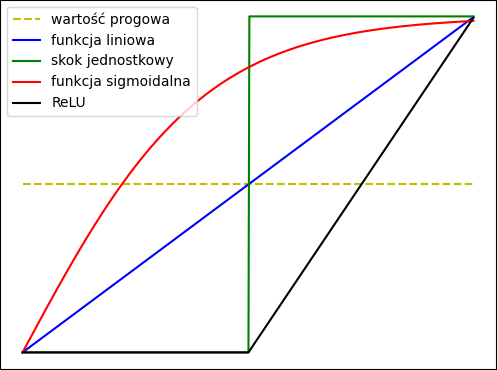
\includegraphics[scale=0.92]{img/aktywacje1.png}        
    \end{center}
    \caption{Funkcje aktywacyjne}
    \label{fig:aktywacje}
\end{figure}


\subsubsection{Perceptron wielowarstwowy (MLP)}

Liczba klas, wobec których perceptron może generalizować jest ograniczona liczbą neuronów w jego warstwie wyjściowej. Oprócz samej liczby neuronów, możemy również zwiększyć ilość warstw perceptronu. Tym sposobem otrzymujemy architekturę \textbf{perceptronu wielowarstwowego}. Jest to, na ten moment, najpopularniejsza architektura sieci neuronowej. Jej schemat przedstawia rysunek \ref{fig:sieć neuronowa}. Składa się ona z jednej warstwy wejściowej, warstw ukrytych złożonych z neuronów McCullocha-Pittsa oraz warstwy wyjściowej. (\ref{itm:warstwy})

Proces uczenia nadzorowanego modelu perceptronu wielowarstwowego jest możliwy dzięki zastosowaniu \textbf{propagacji wstecznej}. To mechanizm polegający na manipulacji wag w celu minimalizacji \textbf{funkcji kosztu}. Często przyjmowaną funkcja kosztu jest błąd średnio-kwadratowy (MSE).

\begin{description}

    \item"\null{}Algorytm \textbf{wstecznej propagacji błędów} polega na takiej zmianie wag sygnałów wejściowych każdego neuronu w każdej warstwie, by wartość błędu dla kolejnych par uczących zawartych w zbiorze uczącym była jak najmniejsza. W tym celu wykorzystywana jest metoda gradientowa najszybszego spadku.
    Schemat krokowy można przedstawić następująco:
    \begin{enumerate}
        \item Inicjalizacja sieci i algorytmu
        \item Obliczanie wartości wyjściowej sieci na podstawie danych
        \item Obliczanie błędu sieci
        \item Korekcja wag
        \item Czy sieć nauczona?
        \item TAK – przejdź dalej
        \item NIE – wróć do punktu 2
        \item Koniec
    \end{enumerate}

    \item Przebieg algorytmu dla wszystkich elementów ciągu uczącego nazywa się \textbf{epoką}." \cite{webarchive}
\end{description}

Funkcja kosztu dana jest ona wzorem:
\begin{center}
\begin{math}
\resizebox{0.42\hsize}{!}{$%
    MSE = \frac{1}{2m}\sum_{i = 1}^{m} ({y}' - y)^{2}
    $%
    }%
\end{math}
\end{center}
gdzie\\
$m$ - ilość próbek\\
$i$ - indeks próbki\\
\begin{math}
{y}'
\end{math}
- wynik otrzymany\\
$y$ - wynik oczekiwany\\

\subsubsection{CNN}

\begin{description}
    \item{
        \textbf{Splotowa sieć neuronowa} (z ang. Convolutional Neural Network - CNN) - to algorytm uczenia maszynowego zaprojektowany na podstawie działania \textbf{kory wzrokowej}. 
        
        Podobnie jak infrastruktura kory wzrokowej, splotowa sieć neuronowa bada obraz etapami. W pierwszym etapie, przetwarzanie obrazu odbywa się na relatywnie małych, \underline{lokalnych polach recepcyjnych}. Części obrazu przetwarzane są wtedy przez neurony reagujące na proste bodźce (linie o różnych orientacjach, krawędzie itp.). Wyjście owych neuronów, jest wejściem dla neuronów, aktywowanych bardziej skomplikowanymi zależnościami w obrazie (kształty, klasy obiektów, kolory itd.), uzyskując stopniowo coraz głębsze i bardziej wyrafinowane powiązania między poszczególnymi aspektami obrazu. Z każdym etapem brane są pod uwagę szersze pola recepcyjne. Mogą się one nakładać na siebie, a łącznie konstruują całe pole wzrokowe \cite{cnn_wroc}.
    }
\end{description}

Wzorowane tym mechanizmem splotowe sieci neuronowe składają się z trzech typów warstw:
\begin{itemize}
    \item Splotowe (z ang. convolution) - "pozwalają na ekstrakcję prostych cech w początkowych warstwach sieci, np. rozpoznają krawędzie o różnej orientacji lub różnokolorowe plamy, a następnie plastry, koła w kolejnych warstwach. Każda warstwa konwolucyjna zawiera cały zbiór filtrów (np. 8 filtrów), a każdy z nich generuje osobną mapę aktywacji 2D. Układamy te mapy aktywacyjne na stercie wzdłuż wymiaru głębokości sieci i produkujemy obraz wyjściowy." \cite{cnn_agh}
    \item Łączące (z ang. pooling) - "\null{}służy do progresywnej redukcji rozmiaru przestrzennego do
zredukowania ilości cech i złożoności obliczeniowej sieci" \cite{cnn_agh}
    \item W pełni połączone lub gęste (FC z ang. fully connected lub dense) - w pełni połączone warstwy, na wzór wielowarstwowego perceptronu.
\end{itemize}

\begin{figure}[h!]
    \begin{center}
        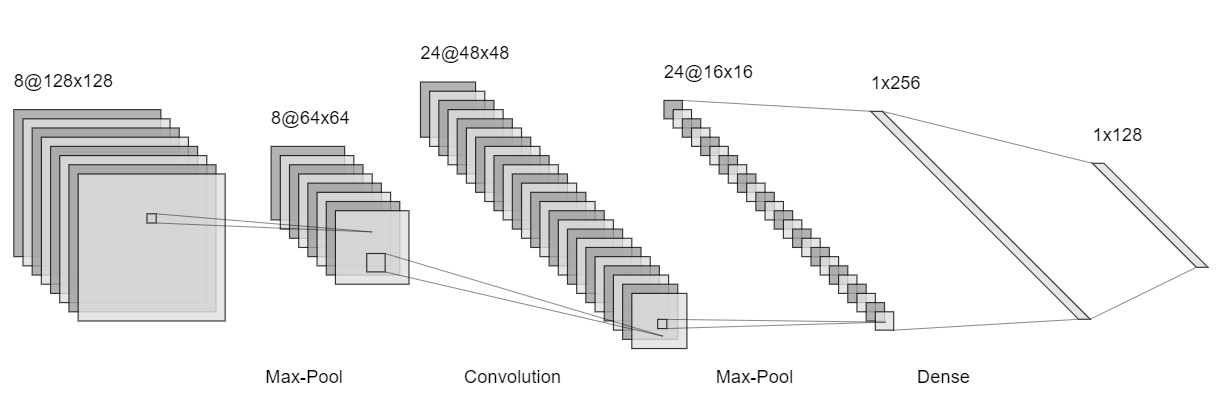
\includegraphics[scale=0.5]{img/cnn_arch_pic.png}
    \end{center}
    \caption{Architektura splotowej sieci neuronowej\protect\footnotemark}
    \label{fig:cnn_arch_pic}
\end{figure}

\footnotetext{Obraz wygenerowany dzięki narzędziu dostępnemu pod adresem: https://alexlenail.me/NN-SVG}

Splotowe sieci neuronowe, tak jak kora wzrokowa, powstały z myślą o danych dwu-wymiarowych (najczęściej obrazy) i właśnie dla tego typu danych są dominującym rozwiązaniem w sferze uczenia maszynowego. W warstwach splotowych wykonywana jest operacja splotu obrazu wejściowego z filtrami, które są przez sieć dostosowywane w celu pozyskania z obrazu poszczególnych cech.

Splotowe sieci neuronowe same w trakcie swojego działania dokonują wyodrębniania cech znaczących. To poważnie zmniejsza liczbę operacji wymaganych w celu optymalizacji ich działania (pozostaję np. selekcjonowanie zbioru danych). Dodatkowo, dzięki swojej architekturze sieci te, wymagają podania mniejszej ilości parametrów w celu konfiguracji. Te dwa fakty znacznie zwiększają przychylność takiego rozwiązania, chociażby ze względu na relatywnie niski wysiłek potrzebny do ich uruchomienia oraz użycia.

Wadą splotowych sieci neuronowych jest to, że przez skomplikowanie i zawarcie w procesie działania wielu złożonych operacji, sieci splotowe są bardzo wolne i wymagające sprzętowo w porównaniu z innymi formami uczenia maszynowego.

Splotowe sieci neuronowe są powszechnie używane w podobnych rozwiązaniach z racji na przystosowanie do danych obrazowych. Na tej technologii oparte są również bardziej skomplikowane i wyrafinowane architekury i modele uczenia maszynowego, na przykład wydajna sieć YOLO (z ang. You Only Look Once) \cite{yolov3}.

\begin{figure}[h!]
    \begin{center}
        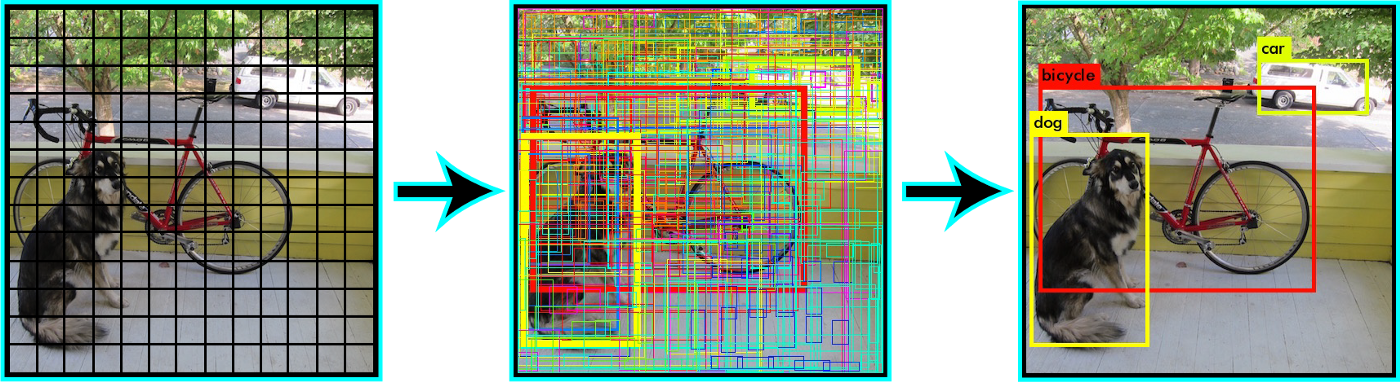
\includegraphics[scale=0.338]{img/yolo_vis.png}
    \end{center}
    \caption{Wizualizacja działania modelu YOLOv3 \cite{yolo_vis}}
    \label{fig:yolo_vis}
\end{figure}
 
 \pagebreak
 
\subsection{Wstępne przetwarzanie danych}
Sieci neuronowe oparte o architekturę perceptronu wielowarstwowego to sieci głębokie, o w pełni połączonych warstwach. Ich wadą jest znaczny wzrost zapotrzebowania na moc obliczeniową oraz pamięć operacyjną wraz z wzrostem liczby parametrów wejściowych. Możemy jednak w dużym stopniu ograniczyć wymogi sprzętowe stosując przetwarzanie danych wejściowych, jeszcze zanim będą one propagowane na wejście sieci. Techniki przetwarzania wstępnego to na przykład: wycinanie, pod-próbkowanie czy wyodrębnianie cech znaczących.

Oprócz tego, realne dane wejściowe, mogą nie być wiernym odwzorowaniem danych uczących. Zdjęcia ruchu ulicznego z reguły mogą zawierać obraz całej drogi i jej okolic, z wieloma pojazdami lub żadnym. Wykrycie pożądanych obiektów jest możliwe dzięki zastosowaniu detekcji obiektów.

\subsubsection{Metody detekcji obiektów}
\begin{description}
\item \textbf{Klasyfikacja} - nadanie etykiety wykrytemu obiektowi, mówiącej do jakiej klasy należy.  

\begin{figure}[h!]
    \begin{center}
        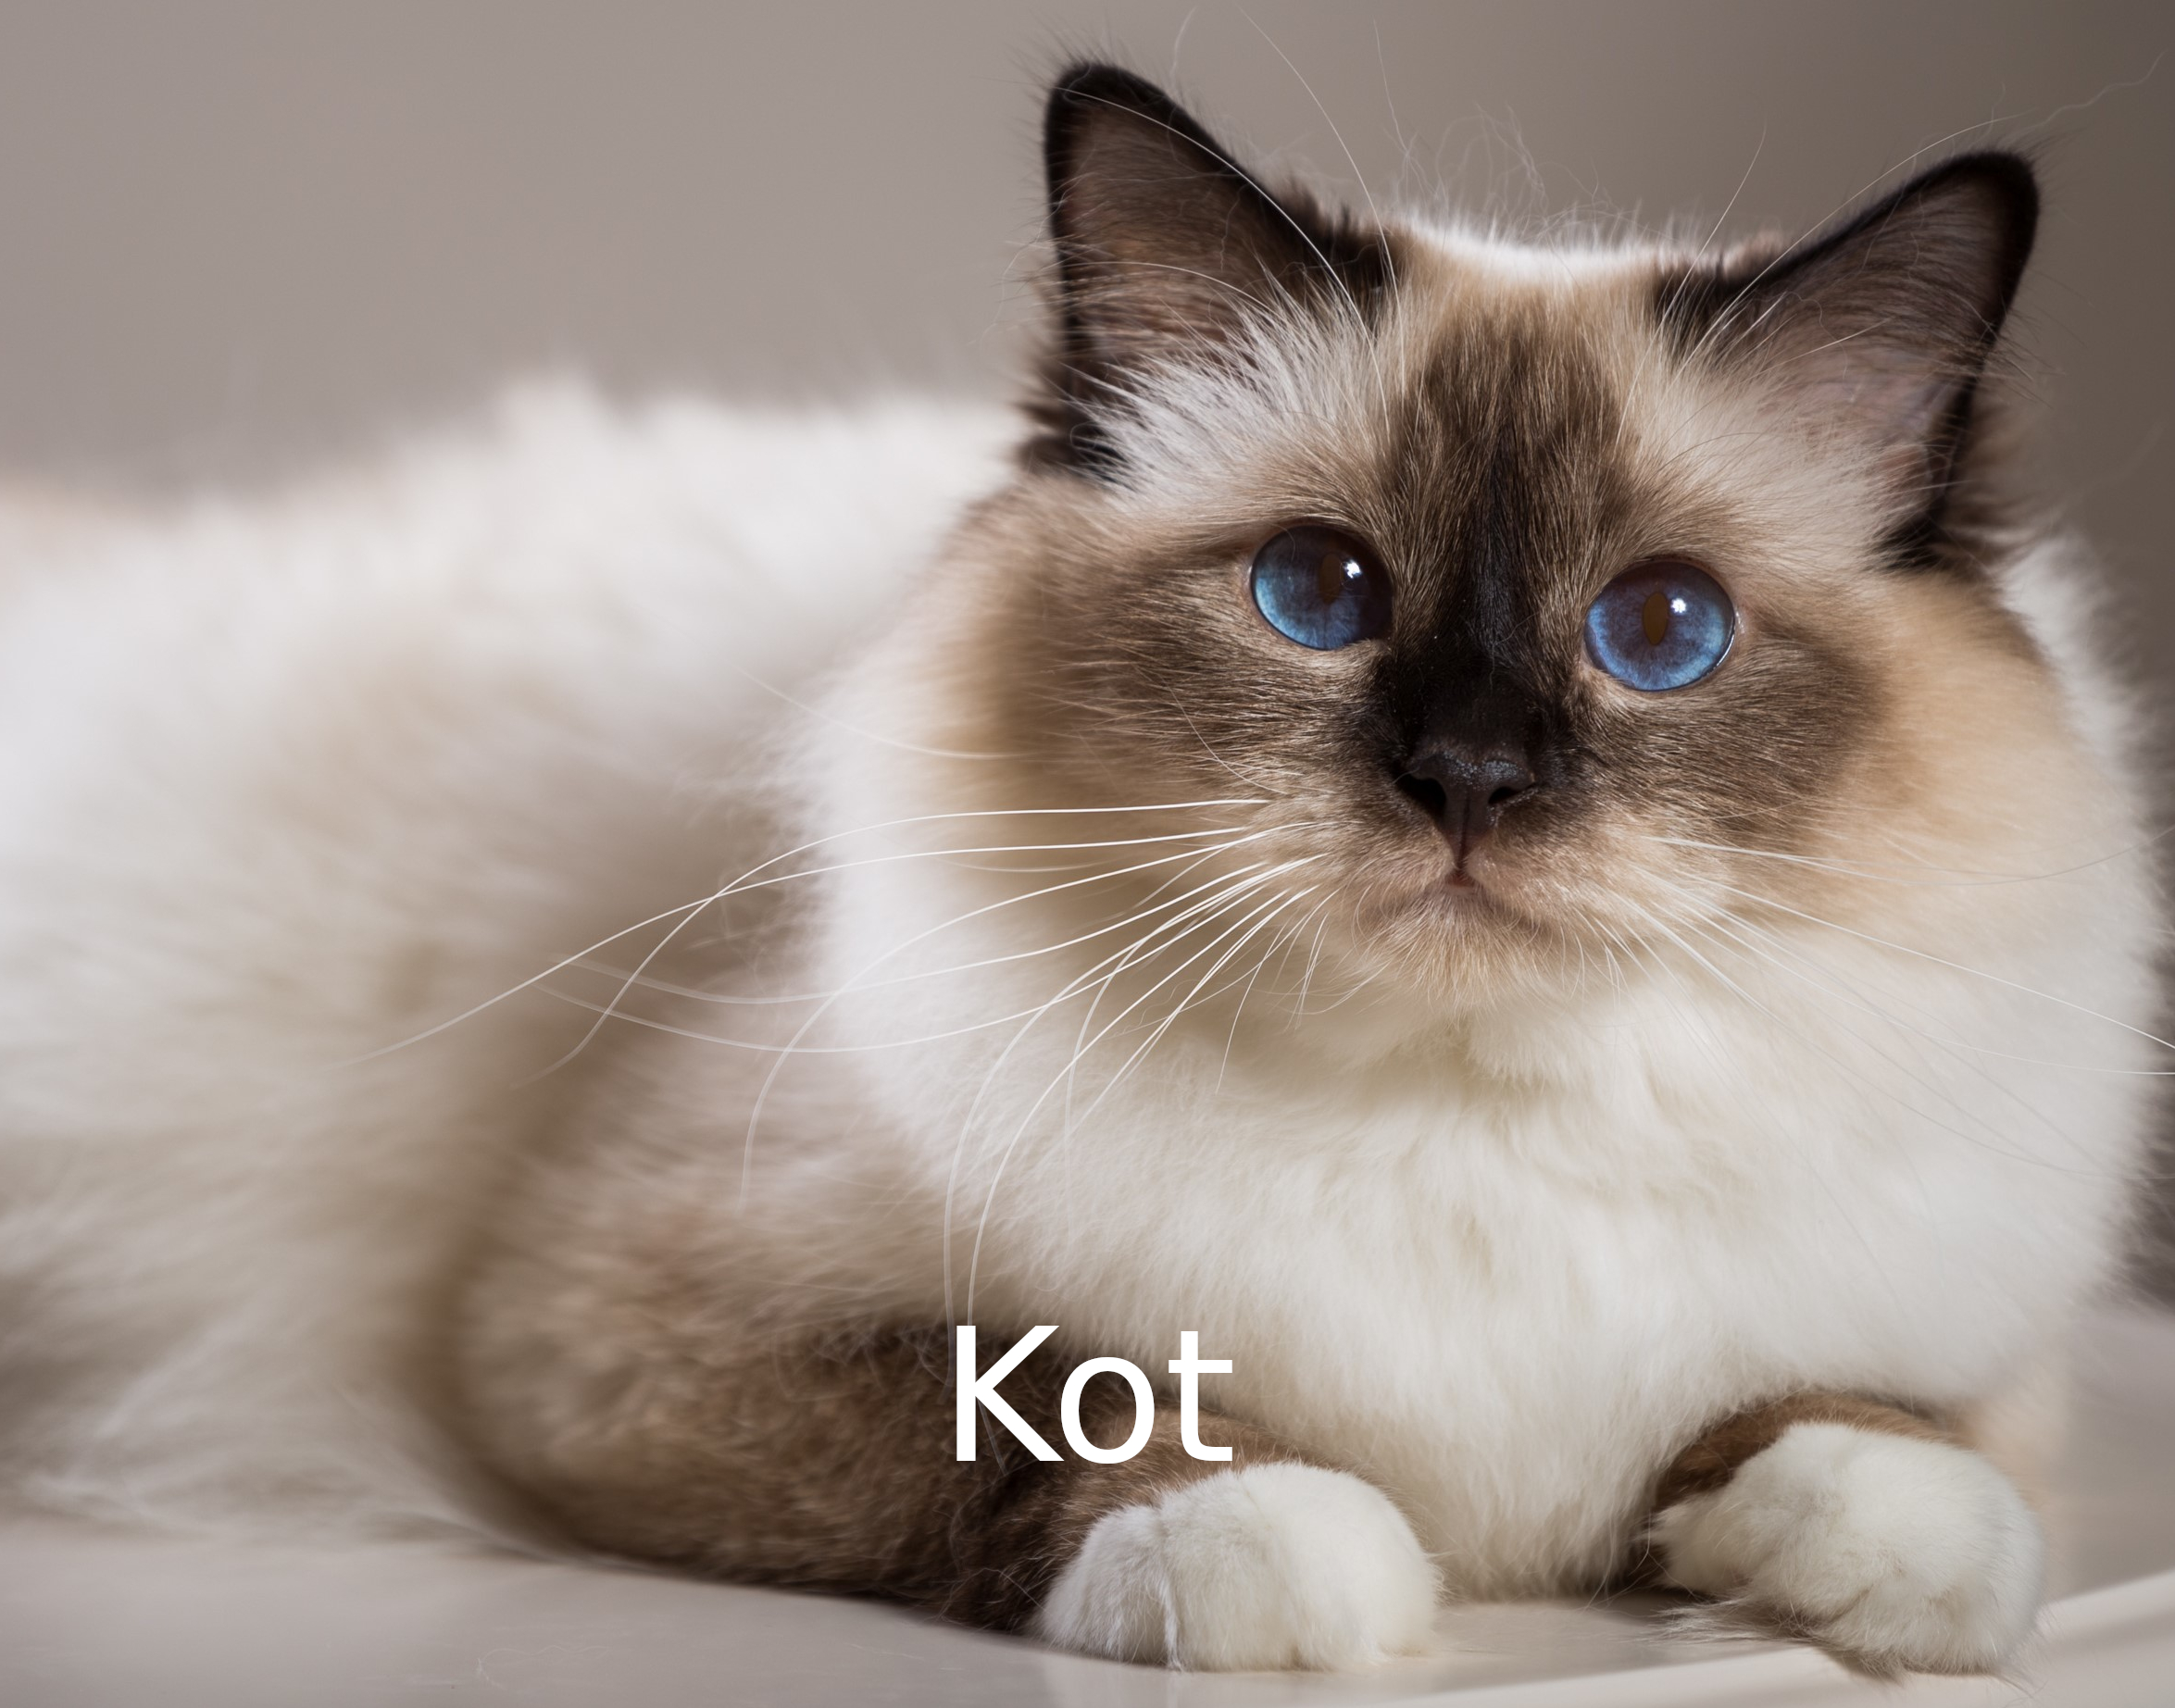
\includegraphics[scale=0.5]{img/kot.jpg}
    \end{center}
    \caption{Wizualizacja klasyfikacji\protect\footnotemark}
    \label{fig:classification_cat}
\end{figure}

\footnotetext{Użyte zdjęcie kota dostępne pod adresem:      \url{https://rikoland.pl/data/include/img/news/1594756840.jpg}}

\item \textbf{Detekcja} - klasyfikacja obiektu wraz z określeniem jego położenia w obrazie, z reguły wizualizowana za pomocą prostokąta opisanego na obwiedni klasyfikowanego podmiotu.

    \begin{figure}[h!]
    \begin{center}
        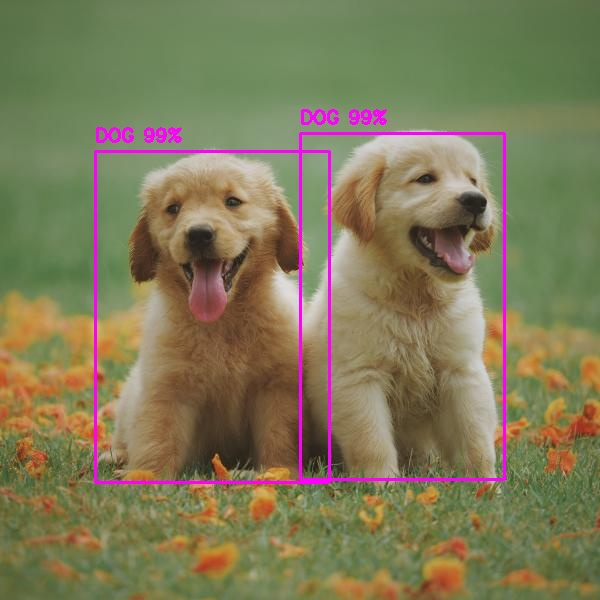
\includegraphics[scale=0.6]{img/detekcja.jpg}
    \end{center}
    \caption{Wizualizacja detekcji\protect\footnotemark}
    \label{fig:detection}
    \end{figure}
    
\footnotetext{Użyte zdjęcie szczeniąt dostępne pod adresem:      \url{https://firsttimedogmom.com/wp-content/uploads/2018/07/Male-vs-Female-Golden-retriever-3.jpg}}

\pagebreak

\item \textbf{Segmentacja} - "proces podziału obrazu na części określane jako obszary (regiony), które są jednorodne (homogeniczne) pod względem pewnych wybranych własności. Obszarami są zbiory pikseli (punktów). Własnościami, które są często wybierane jako kryteria jednorodności obszarów są: poziom szarości, barwa, tekstura." (lub klasy) \cite{wikiseg}.

Segmentacje można podzielić na:
    \begin{itemize}
        
        \item \textbf{Semantyczną} - to rozróżnienie obrazu na segmenty, przy czym obiekty należące od tej samej klasy nie są między sobą rozróżniane. 
        
        \item \textbf{Instancji} - działa jak segmentacja semantyczna, z tą różnicą, że poszczególne instancje tej samej klasy są rozróżniane.
        
    \end{itemize}

    \begin{figure}[h!]
    \begin{center}
        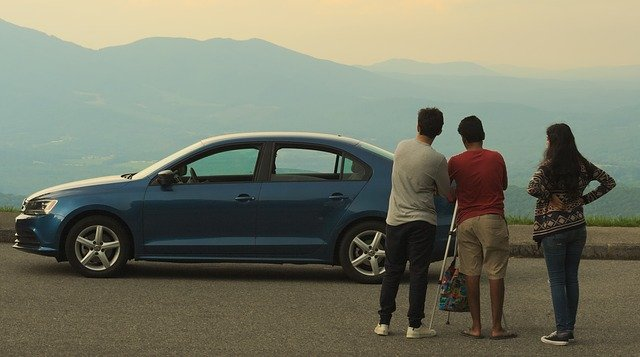
\includegraphics[scale=0.5]{img/car_people.jpg}
    \end{center}
    \caption{Obraz referencyjny\protect\footnotemark}
    \label{fig:ref_seg}
    \end{figure}
    
    \footnotetext{Użyte zdjęcie referencyjne dostępne pod adresem: \url{https://cdn.pixabay.com/photo/2018/04/17/21/56/car-3328898_960_720.jpg}}
    
    \begin{figure}[h!]
    \begin{center}
        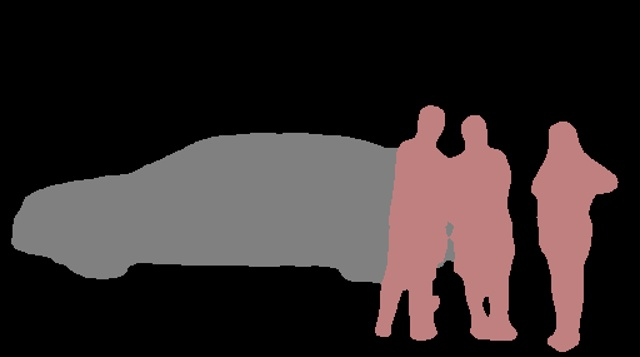
\includegraphics[scale=0.5]{img/car_people_sem.jpg}
    \end{center}
    \caption{Wizualizacja segmentacji semantycznej}
    \label{fig:seg_sem}
    \end{figure}
    
    \begin{figure}[h!]
    \begin{center}
        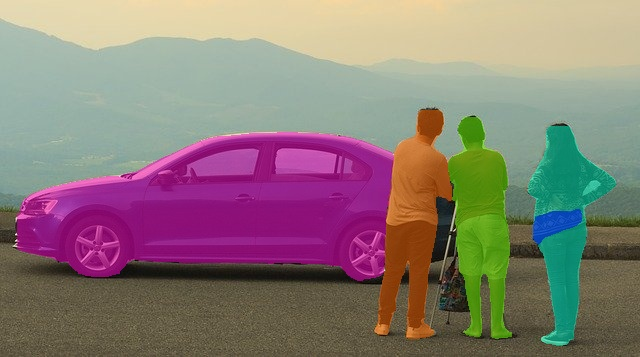
\includegraphics[scale=0.5]{img/car_people_ins.jpg}        
    \end{center}
    \caption{Wizualizacja segmentacji instancji w formie maski nałożonej na obraz referencyjny}
    \label{fig:seg_ins}
    \end{figure}
    
\end{description}

\pagebreak

\subsubsection{Wyodrębnianie cech znaczących}

\textbf{Cechy znaczące} - to wyselekcjonowane części danej wejściowej, na podstawie której model ma wywnioskować potencjalny wynik. Stosujemy konstrukt cech znaczących, aby zniwelować szum mogący powstać przez wpływ niekorzystnych lub nieinteresujących nas elementów wejścia.\\

\begin{figure}[h!]
    \begin{center}
        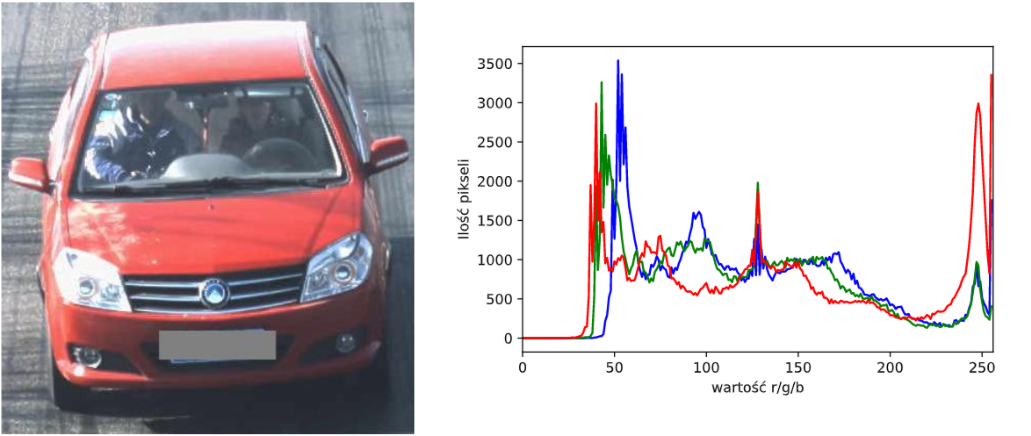
\includegraphics[scale=0.6]{img/feature_extraction.png}        
    \end{center}
    \caption{Ekstrakcja cech znaczących w postaci histogramu kolorów}
    \label{fig:ekstrakcja}
\end{figure}

Wyodrębnianie cech znaczących jest stosowane w celu zmniejszenia wymiarowości napotkanego problemu. W przypadku obrazów wiąże się z ich obróbką, bądź odizolowaniem z nich poszczególnych elementów.

Popularnymi sposobami ekstrakcji cech znaczących są:

\begin{itemize}
    \item Maskowanie elementów obrazu
    \item Wykrywanie obwiedni
    \item Wykrywanie obszarów jednolitych 
    \item Wykrywanie ruchu
    \item Transformacja Hougha i jej pochodne - metoda odszukiwania regularnych kształtów (oryginalnie prostych)
    \item Filtrowanie (w tym górno oraz dolnoprzepustowe)
    \item Dopasowywanie wzorcowe
\end{itemize}


\subsection{Statystyka dotycząca kolorów aut na polskich drogach}

Gama kolorów aut jest bardzo szeroka. Jednak jest ona zdominowana przez kilka najpopularniejszych barw.

Czołowa dziesiątka najpopularniejszych kolorów \cite{autocentrum}:
\begin{enumerate}
    
    \item Srebrny – 25\%
    \item Czarny – 23\%
    \item Biały – 16\%
    \item Szary – 13\%
    \item Niebieski – 9\%
    \item Czerwony – 8\%
    \item Brązowy i beżowy – 4\%
    \item Zielony – 1\%
    \item Żółty i złoty – 1\%
    \item Inne – poniżej 1\% 
\end{enumerate}

Wyciągając dalsze wnioski z owej statystyki, można zauważyć, że biorąc pod uwagę jedynie osiem kolorów: srebrny, czarny, biały, szary, niebieski, czerwony, cyjanowy, zielony i żółty - otrzymamy ponad \textbf{93\%} pokrycia barw wszystkich aut. Właśnie te kolory są dostępne w użytym zbiorze danych.

Kolory srebrny i szary są uwzględnione jako jeden kolor z uwagi na trudność ich rozróżnienia. Zdjęcia w zbiorze danych borykają się z wieloma problemami wpływającymi znacznie na ich jakość (opisane dogłębnie w podrozdziale \ref{sec:dataset}). Metaliczny połysk srebra jest niemal zawsze w warunkach drogowych zatracany przez brud, kurz, warunki atmosferyczne, oświetlenie i jakość zdjęć. To sprawia, że w większości przypadków, te dwa kolory są nierozróżnialne z punktu widzenia ludzkiego oka, a tym bardziej programowo.

\subsection{Użyty zbiór danych}
\label{sec:dataset}

Dane użyte do trenowania modelu uczenia maszynowego pochodzą z publikacji naukowej dotyczącej tematyki rozpoznawania koloru aut \cite{chen_ref}.\\

Zbiór danych składa się z 15601 obrazów przedstawiających pojazdy na drogach miejskich widziane od przodu. Zdjęcia zostały wykonane przy pomocy kamery o rozdzielczości 1920x1080.

\begin{figure}[h!]
    \begin{center}
        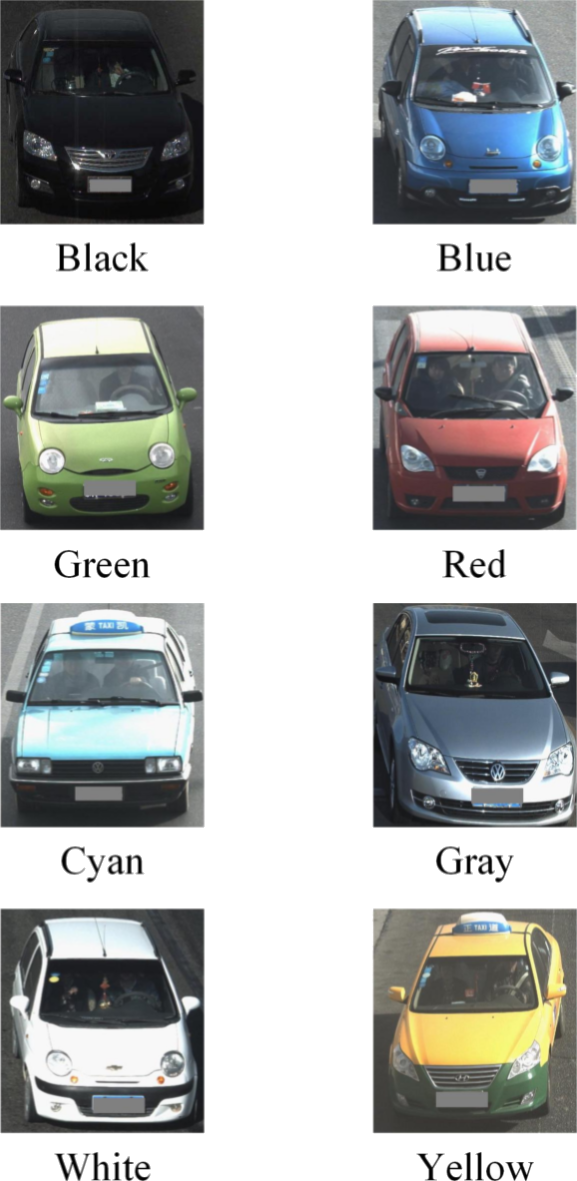
\includegraphics[scale=0.73]{img/dataset.png}        
    \end{center}
    \caption{Przykładowe obrazy ze zbioru danych wraz z ich etykietami}
    \label{fig:przykładowe obrazy}
\end{figure}

\pagebreak

Zbiór jest obarczony wieloma problemami wpływającymi na wynikowe działanie trenowanego nim modelu:

\begin{itemize}
    \item Składa się jedynie ze zdjęć pojazdów z widoku frontalnego, co sprawia, że model optymalnie wywnioskuje jedynie samochody widziane z podobnej perspektywy. Przez to jest ograniczony.
    \item Część zdjęć jest widocznie zniekształcona przez zastałe warunki atmosferyczne, oświetlenie oraz wszelakiego rodzaju rozmycie obrazu. Przez to, rozróżnienie par kolorów zbliżonych do siebie (na przykład szary-czarny i szary-biały) jest problematyczne.
    \item Obrazy zawierają w sobie element tła, którego negatywny wpływ na ekstrahowany histogram kolorów jest zauważalny w wynikowym działaniu algorytmu. Programowe usunięcie tła to bardzo kosztowna operacja pod względem zasobów. Jest to szczególnie dotkliwe dla wydajności przy działaniu programu na plikach wideo.
    \item Niektóre zdjęcia, przez prawdopodobny wpływ czynnika ludzkiego w procesie manualnej klasyfikacji, mają niepoprawnie przypisane kolory.
    \item W zbiorze istnieją zdjęcia pojazdów, których elementy karoserii są różnych kolorów. Fakt ten sprawia, iż wyuczony model może zostać zdegenerowany przez zawarcie w histogramach kolorów innej barwy, niż koloru przypisanego do danego zdjęcia.
\end{itemize}

% \subsection{Informacja o kolorze pozyskiwana z obrazu}

% Informacje o obrazie w postaci numerycznej można pozyskać dzięki użyciu biblioteki OpenCV w języku Python.
% Metoda \textbf{cv2.imread()} zwraca informacje o wartościach kanałów \textbf{RGB} każdego piksela w postaci zagnieżdżonej listy. Wykaz wspieranych formatów obrazów metody jest liczny, a co ważniejsze zawiera w sobie formaty \textbf{.jpg} oraz \textbf{.png}. Jest również możliwe użycie OpenCV do przetworzenia na dane numeryczne plików wideo, między innymi \textbf{.mp4} i \textbf{.avi}.

% \begin{lstlisting}[language=Python, caption=Przykład wczytania obrazu]
% import cv2  # Korzystamy z biblioteki openCV

% file_path = r'../assets/0197.jpg'
% image = cv2.imread(file_path)

% print(image.shape)
% print(image)
% \end{lstlisting}


% \begin{lstlisting}[language=Python, caption=Wynik wczytania obrazu]
% (426, 408, 3)  # wymiary obrazu (426, 408) oraz kanaly RGB (3)
% [[[193 185 178]  # Tablica wartosci kanalow RGB poszczegolnych pikseli
%   [202 194 187]  
%   [204 196 189]
%   ...
%   [131 127 116]
%   [132 128 117]
%   [132 128 117]]]
% \end{lstlisting}

% \begin{lstlisting}[language=Python, caption=Wizualizacja wczytanego obrazu]
% import cv2

% file_path = r'../assets/0197.jpg'
% image = cv2.imread(file_path)  # Wczytanie obrazu

% cv2.imshow('Window title', image)  # Wyswietlenie obrazu w oknie o tytule 'Window title'
% cv2.waitKey(0)  # Instrukcja wstrzymujaca zamkniecie okna z obrazem az uzytkownik kliknie dowolny przycisk
% \end{lstlisting}

% \begin{figure}[h!]
%     \begin{center}
%         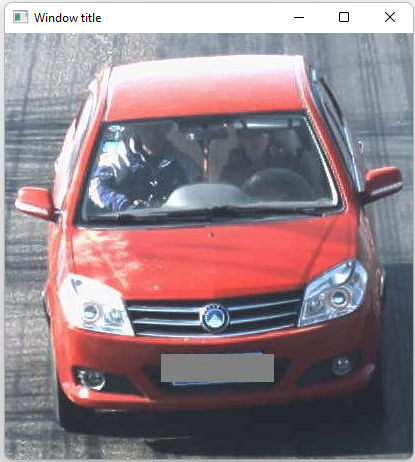
\includegraphics[scale=1.1]{img/0197-windowed.png}        
%     \end{center}
%     \caption{Wczytany obraz pokazany w oknie}
%     \label{fig:wczytanie obrazu}
% \end{figure}

% \pagebreak

% Do wczytywania plików wideo lub obrazu na żywo z wejścia wideo komputera używamy klasy \textbf{cv2.VideoCapture()}. Wczytujemy dzięki niej kolejne klatki pliku wideo. Wynik wczytania każdej z klatek jest tożsamy do wyniku funkcji \textbf{cv2.imread()} na pojedynczym obrazie.\\
% Przykład jej użycia:

% \begin{lstlisting}[language=Python, caption=Wczytanie oraz wizualizacja wideo]
% import cv2

% video_file_path = r'../assets/blue_car.mp4'

% cap = cv2.VideoCapture(video_file_path)

% while cap.isOpened():  # Jesli udalo sie otworzyc plik, powtarzaj operacje czytania + przetwarzania + wizualizuj
%     success, img = cap.read()  # Czytaj kolejna klatke

%     # Przerwij petle jesli napotkany zostanie koniec pliku
%     if not success:
%         break

%     # Potencjalne operacje na obrazie

%     cv2.imshow("Window title", img)  # Wyswietl klatke w oknie o tytule  'Window title'
%     cv2.waitKey(1)  # 1 milisekundowa przerwa pomiedzy klatkami 

% cap.release()  # Zwolnij zasoby
% cap.destroyAllWindows()  # Zamknij okna otwarte przez openCV 
% \end{lstlisting}